\chapter{Introduction}
\label{chap:introduction}

\chapterquote{There, sir! that is the perfection of vessels!}
{Jules Verne, 1828--1905}

%========================================================================================

The Standard Model has proven to be one of the greatest accomplishments of modern day particle physics.  It has been used to make countless predictions of various physics processes across a wide range of energies which have proven to be consistent with experimental measurements.  The final piece of the Standard Model to be discovered was the Higgs boson, which was found by the ATLAS \cite{Aad:2012tfa} and CMS \cite{Chatrchyan:2012xdj} experiments at the Large Hadron Collider (LHC) in 2012.  

Despite the remarkable descriptive power of the Standard Model, there are a number of features in the universe that it does not provide a description for.  How does gravity fit into the Standard Model?  Why is there an excess of matter over antimatter in the observable universe?  What is "dark matter" and "dark energy"?  How does "dark matter" couple with the particles in the Standard Model?  What are the properties of the Higgs field in the Standard Model?  While the LHC and previous generations of particle collider experiment have had enormous success in validating the Standard Model and searching for new physics, it is clear that there is more work to be done. 

The linear collider experiments are a set of proposals for the next generation of particle collider experiments.  These experiments are TeV scale $\text{e}^{+}\text{e}^{-}$ colliders with an emphasis on precision measurements.  The physics programme for the linear collider is designed to complement and extend the work done at the LHC and to develop our understanding of particle physics.  One of the primary goals of the linear collider experiments is to study the Higgs field of the Standard Model.  A detailed description of the Higgs field could help in the description of "dark matter" as many extensions of the Standard Model Higgs field contain particles that fit the properties of "dark matter".  The linear collider experiments will also provide a detailed description of the properties of the top quark.  This will complement the Higgs study because the strongest couplings for the Higgs in the Standard Model occurs with the top quark.  Another goal of the linear collider experiments is to provide high precision measurements of the electroweak sector in the Standard Model.  As the electroweak sector is the only place in the Standard Model where CP violation can occur, a detailed description will help to determine why there is an excess of matter over antimatter in the universe.  Furthermore, the linear collider will expand the descriptive reach for many Standard Model extensions such as supersymmetry (SUSY).

As well as searching for beyond Standard Model physics, precision measurements at the linear collider will guide the future direction of experimental particle physics.  Precision measurements have helped to guide the course of particle physics experiments in the past; LEP electroweak data, which gave indirect information about the lightness of the Higgs boson, was used to build the physics case for the LHC.  By colliding electrons and positrons, which are fundamental particles, the experimental conditions found at the linear collider will be far cleaner than those at the LHC, which makes it easier to perform precision measurements.  High precision measurements are made possible at the linear collider due to the use of particle flow calorimetry, a revolutionary technique in calorimetry that offers exceptional energy resolution for jets.  This paradigm shift means the linear collider detectors are significantly different from those found in previous generations of particle colliders.  As the detector design is continually evolving, the ongoing research in this area is vital for determining the overall success of these proposed experiments.  

This thesis is organised as follows.  Chapter \ref{chap:anomalousgaugecouplingtheory} contains a summary of the Standard Model as well as an outline of the physics of interest related to the analysis presented in chapter \ref{chap:PhysicsAnalysis}.  Chapter \ref{chap:clicvertex} presents a study into a novel technology option for the Compact LInear Collider (CLIC) vertex detector.  Chapter \ref{chap:energyestimators} contains numerous studies related to the treatment of energy deposits in the linear collider simulation.  This begins with an outline of the calibration procedure for the linear collider detector simulation.  It is then followed by a number of novel software techniques aimed at improving the energy resolution of a calorimeter designed for particle flow calorimetry.  Finally, chapter \ref{chap:energyestimators} concludes with a study of the timing requirements applied in the software trigger that will be used at the linear collider experiments.  Chapter \ref{chap:detopt} presents an optimisation study of the linear collider calorimeters.  The starkest contrast in detector design, when comparing particle flow calorimetry to tradition calorimetry, is the design of the calorimeters.  As the linear collider experiments will be the first experiments purposefully built with particle flow calorimetry in mind, this study will be vital for guiding detector construction.  Chapter \ref{chap:PhysicsAnalysis} contains a study into anomalous gauge couplings that are sensitive to massive gauge boson quartic vertices at the CLIC experiment.  This study is of particular interest as it provides a detailed probe of the electroweak symmetry breaking sector of the Standard Model as well as showing CLICs sensitivity to a possible extension to the Standard Model.  The thesis concludes with a summary in chapter \ref{chap:summary}.

%========================================================================================

\section{Future Linear Colliders}
There are two proposed future linear colliders; the International Linear Collider (ILC) and the Compact LInear Collider (CLIC).  These colliders are both $\text{e}^{+}\text{e}^{-}$ colliders with focus upon precision measurements, however, they operate at different collision energies, which presents each experiment with its own unique challenges.  One benefit of a linear collider is that it is possible to stage the experiment at several different energies throughout the experiments lifetime

%========================================================================================

\subsection{The International Linear Collider}
The ILC, shown in figure \ref{fig:ilc}, initially plans to operate at a centre-of-mass energy of 250~GeV to study the Higgs boson in detail through the Higgstrahlung process ($\text{e}^{+}\text{e}^{-} \rightarrow ZH$) \cite{Behnke:2013xla}.  The analysis of this process makes it possible to examine all the decays of the Higgs boson with high precision.  The next phase of operation will increase the collision energy to 500~GeV.  This will extend the study of the Higgs, making it possible to observe the Higgs coupling with the top quark and to determine self interactions of the Higgs.  Furthermore, at this energy, it will be possible to search for evidence for SUSY and extended Higgs states.  Finally, there is an option to increase the centre-of-mass up to 1~TeV, further extending the search for SUSY and composite Higgs models.

\begin{figure}[h!]
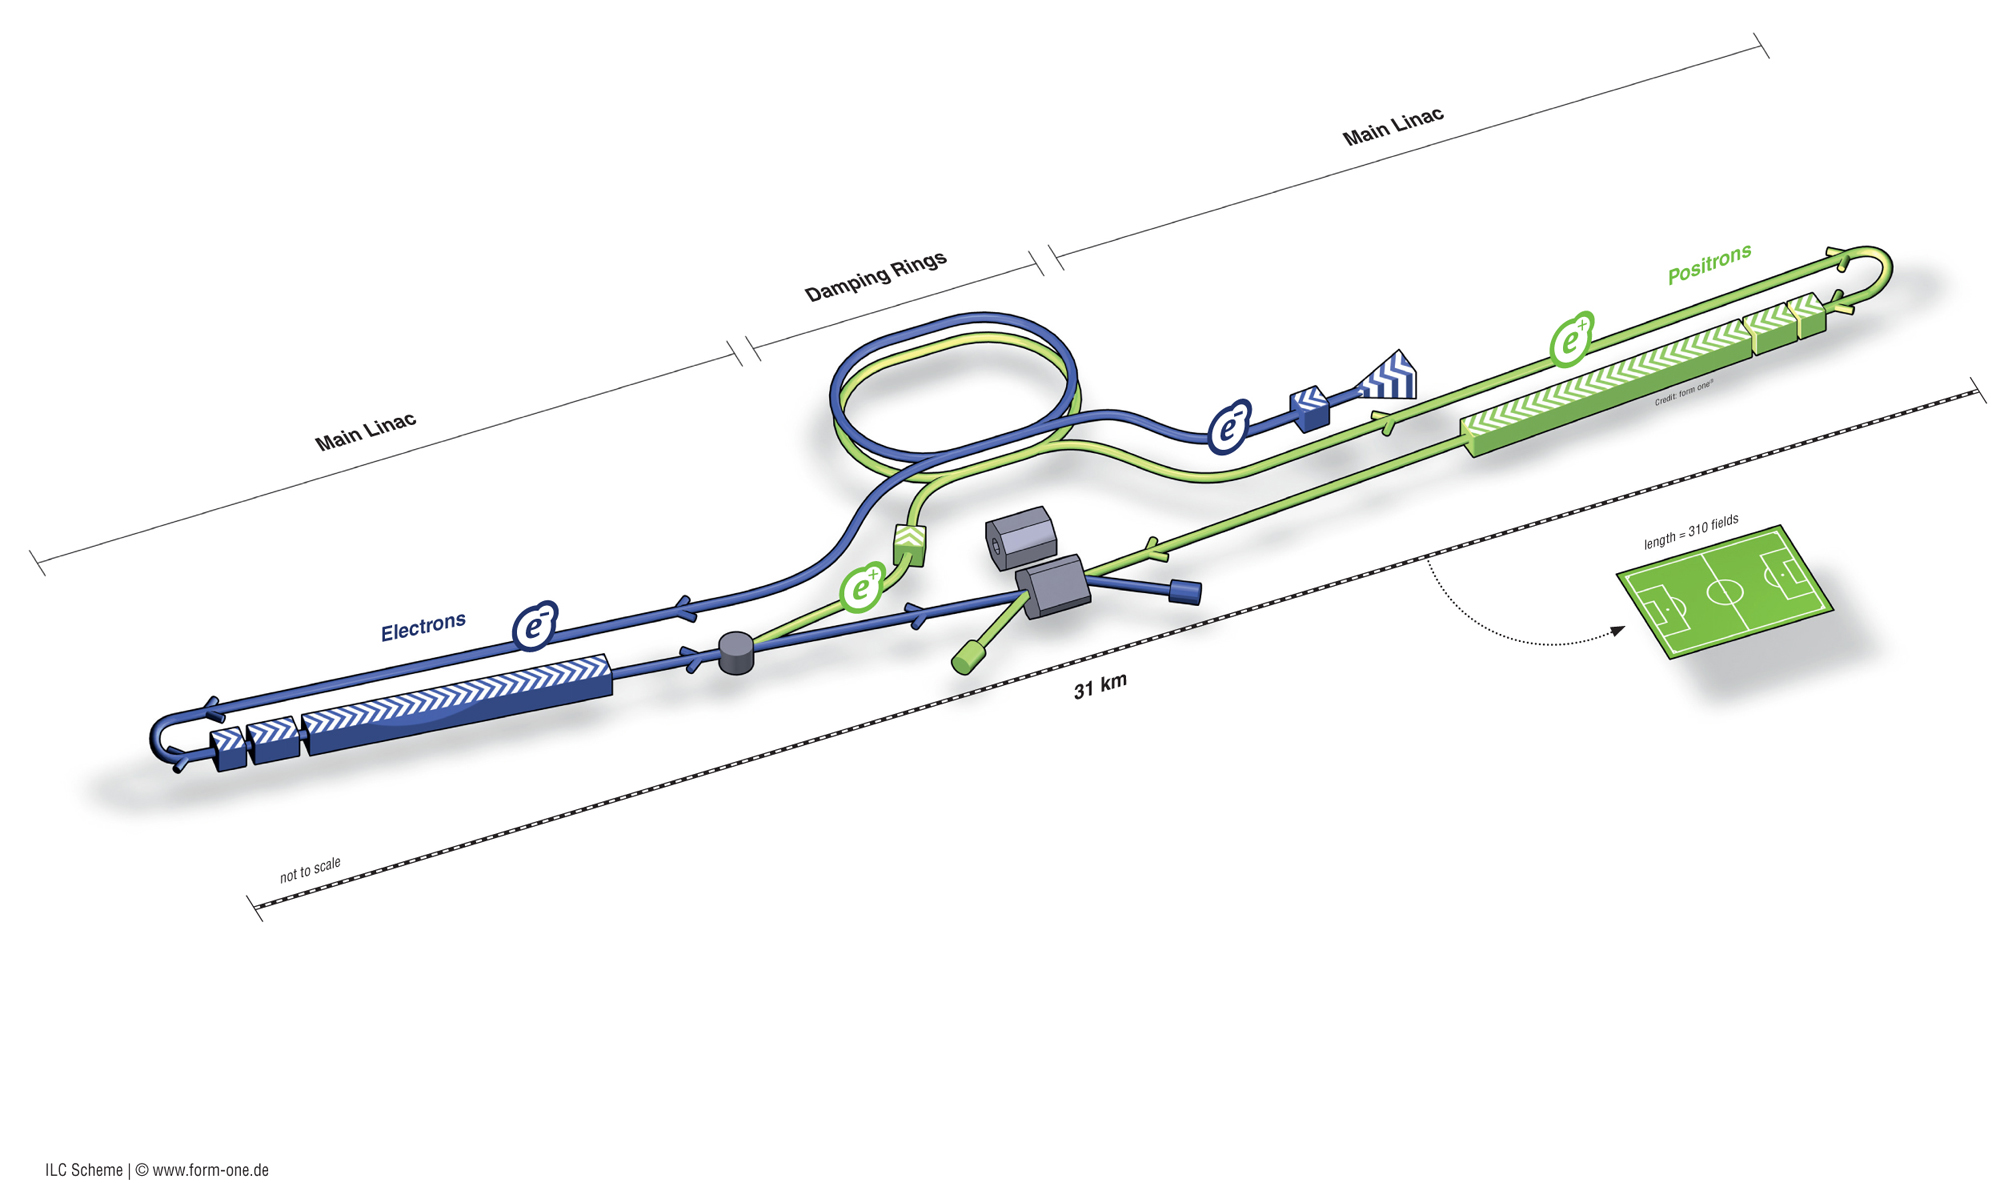
\includegraphics[width=1.0\textwidth]{Introduction/Plots/ILC.jpg}
\caption[Schematic layout of the ILC, indicating all the major subsystems (not to scale).  Figure taken from \cite{Behnke:2013xla}.]{Schematic layout of the ILC, indicating all the major subsystems (not to scale).  Figure taken from \cite{Behnke:2013xla}.}
\label{fig:ilc}
\end{figure}

%========================================================================================

\subsection{The Compact Linear Collider}
The CLIC experiment, shown in figure \ref{fig:clic}, plans to operate with maximum collision energy of 3~TeV \cite{Linssen:2012hp, CLIC:2016zwp}.  CLIC will also operate at intermediate energy stages, however, these energies are to be determined by the ongoing work at the LHC.  The large collision energy of CLIC gives it a greater physics reach to search for extensions to the Standard Model, e.g. SUSY, that would be inaccessible at ILC-like energies.  Although the exact energies for the staging of the CLIC experiment are not certain, CLIC will operate at a low collision energy during staging, 380~GeV, to study the Higgs.  The higher energy stages of the CLIC experiment will provide access to different channels for studying Higgs couplings, as shown by figure \ref{fig:higssprodclic}.

\begin{figure}[h!]
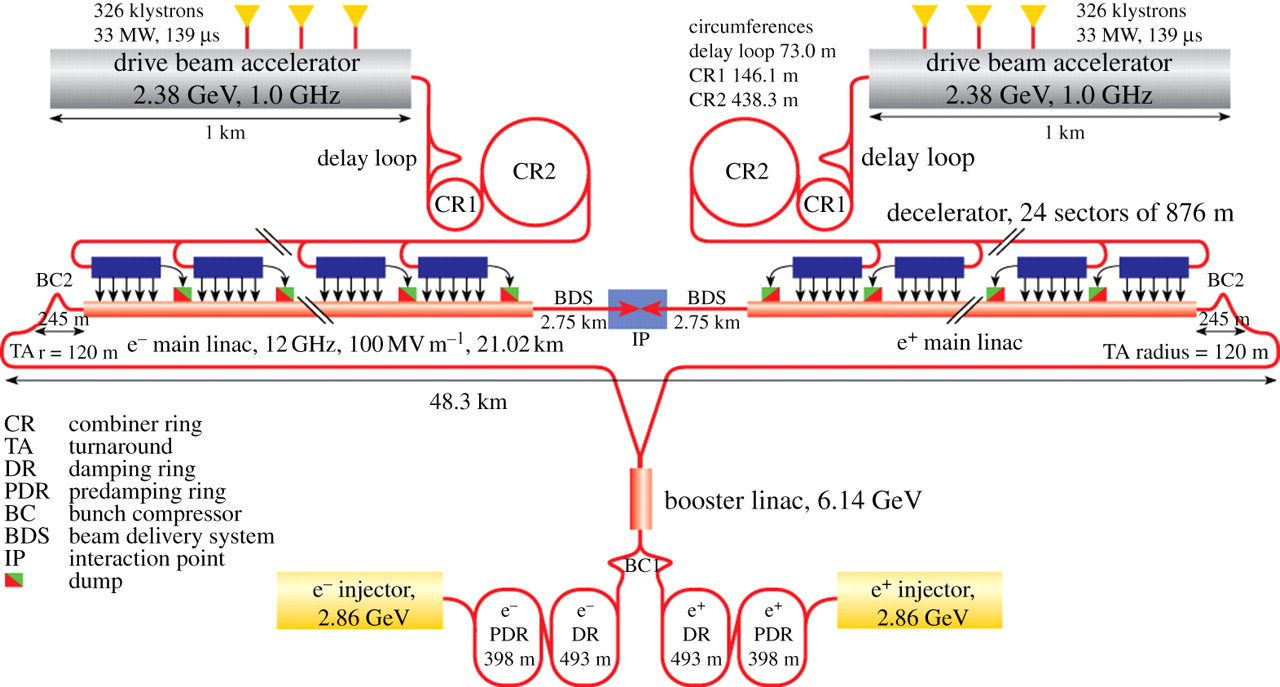
\includegraphics[width=1.0\textwidth]{Introduction/Plots/CLIC.jpg}
\caption[CLIC layout at 3~TeV.  Figure taken from \cite{Aicheler:2012bya}.]{CLIC layout at 3~TeV.  Figure taken from \cite{Aicheler:2012bya}.}
\label{fig:clic}
\end{figure}

\begin{figure}[h!]
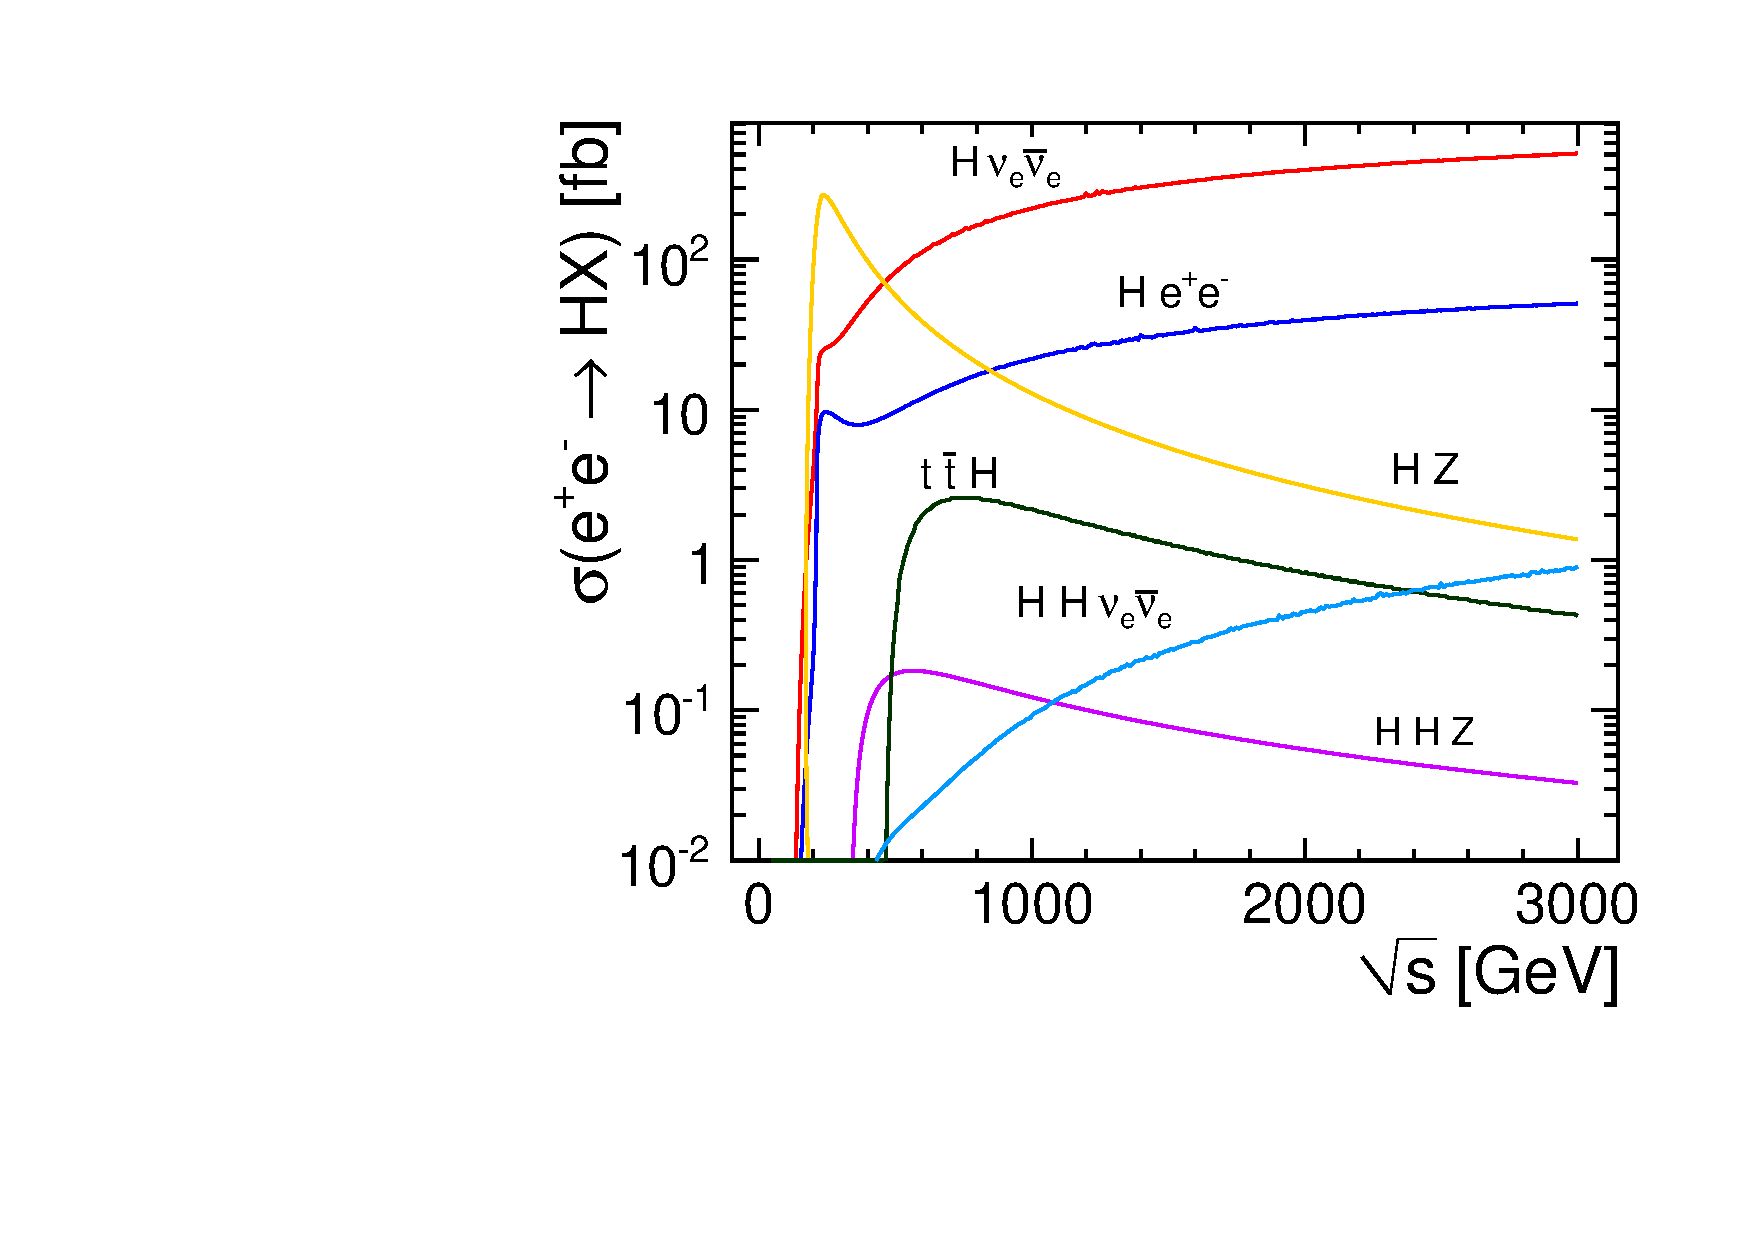
\includegraphics[width=0.5\textwidth]{Introduction/Plots/CDRPlots/HiggsCrossSectionCLIC.pdf}
\caption[Cross section for production mechanisms of the Standard Model Higgs boson as a function of the collision energy.  The cross sections were calculated assuming a Higgs mass of 120~GeV.  Figure taken from \cite{Linssen:2012hp}.]{Cross section for production mechanisms of the Standard Model Higgs boson as a function of the collision energy.  The cross sections were calculated assuming a Higgs mass of 120~GeV.  Figure taken from \cite{Linssen:2012hp}.}
\label{fig:higssprodclic}
\end{figure}

%========================================================================================

\subsubsection{Experimental Conditions at CLIC}
The CLIC experiment will operate in a unique environment in comparison to either the ILC or previous generations of lepton colliders.  It is vital that this is properly accounted for when determining the physics potential that CLIC has to offer.  The following aspects of the CLIC experiment present the largest challenges to the physics potential:

\begin{itemize}
\item \textbf{The high bunch charge density}.  The small beam size at the impact point produces very large electromagnetic fields.  These fields can interact with the opposite beam particles causing them to radiate photons in an effect known as beamstrahlung.  Beamstrahlung acts to reduce the collision energy of the $\text{e}^{+}\text{e}^{-}$ pairs.   
\item \textbf{Beam related backgrounds}.  Beamstrahlung photons can subsequently interact to produce background events that must be accounted for.  Dominant backgrounds of this form that cannot be easily vetoed in the reconstruction include incoherent pair production of $\text{e}^{+}\text{e}^{-}$ and $\gamma\gamma \rightarrow hadrons$.  While these backgrounds are also problematic for the ILC experiment, the lower collision energy means it is has a much smaller impact on performance.
\item \textbf{Fast readout technology}.  The CLIC bunch train consists of 312 bunches with a repetition rate of 50~Hz.  Each bunch is separated by 0.5~ns, therefore, it will be necessary to integrate over multiple bunch crossing when reading out the detectors.  This places tight constraints on all detector electrical readout speeds and time resolutions.   
\end{itemize}

%========================================================================================

\subsubsection{Beam-Related Backgrounds at CLIC}
\label{sec:beamrelatedbackgrounds}
The primary sources of background for the CLIC experiment are as follows:
\begin{itemize}
\item $\text{e}^{+}\text{e}^{-}$ pair creation from the interaction of a beamstrahlung photons with the opposing beam.  The different mechanisms for pair creation are as follows:
\begin{itemize}
\item \textbf{Coherent pair production}: the interaction of a real beamstrahlung photon with the electromagnetic field from the opposing beam.
\item \textbf{Trident pair production}: the interaction of a virtual beamstrahlung photon with the electromagnetic field from the opposing beam.
\item \textbf{Incoherent pair production}: the interaction of a real or virtual beamstrahlung photon with the individual particles in the opposing beam.
\end{itemize}
\item $\gamma\gamma \rightarrow hadrons$ events from the interaction of real or virtual beamstrahlung photons with each other.  
\item Beam halo muons that arise from interactions of the beam particles during collimation.  The dominant mechanisms producing beam halo muons are photon conversions into muon pairs ($\gamma \text{e}^{-} \rightarrow \mu^{+}\mu^{-}\text{e}^{-}$) and annihilation of positrons with atomic $\text{e}^{-}$ into muon pairs ($\text{e}^{+}\text{e}^{-} \rightarrow \mu^{+}\mu^{-}$) \cite{Pilicer:2015ijy}.
\end{itemize}

These backgrounds must be properly addressed to get a true measure of the physics potential CLIC has to offer.  Coherent and trident pair production are not dominant sources of background because they have low transverse momenta and are collinear with the outgoing beam, as figure \ref{fig:backgroundangle} shows.  This is not the case for incoherent pair production of $\text{e}^{+}\text{e}^{-}$, which is dominant in the forward regions of the detector, and $\gamma\gamma \rightarrow hadrons$, which is dominant in the tracker and the calorimeters (with the exception of low radii in the calorimeter endcaps) \cite{Linssen:2012hp, Sailer:2012mfa}.  Beam halo muons are not a major source of background either as they can be easily removed during the reconstruction since they produce a clear signal in the detector.  An algorithm was developed within the PandoraPFA framework for this purpose and it was found to be highly effective at removing the beam halo muon backgrounds \cite{Linssen:2012hp}.  

\begin{figure}[h!]
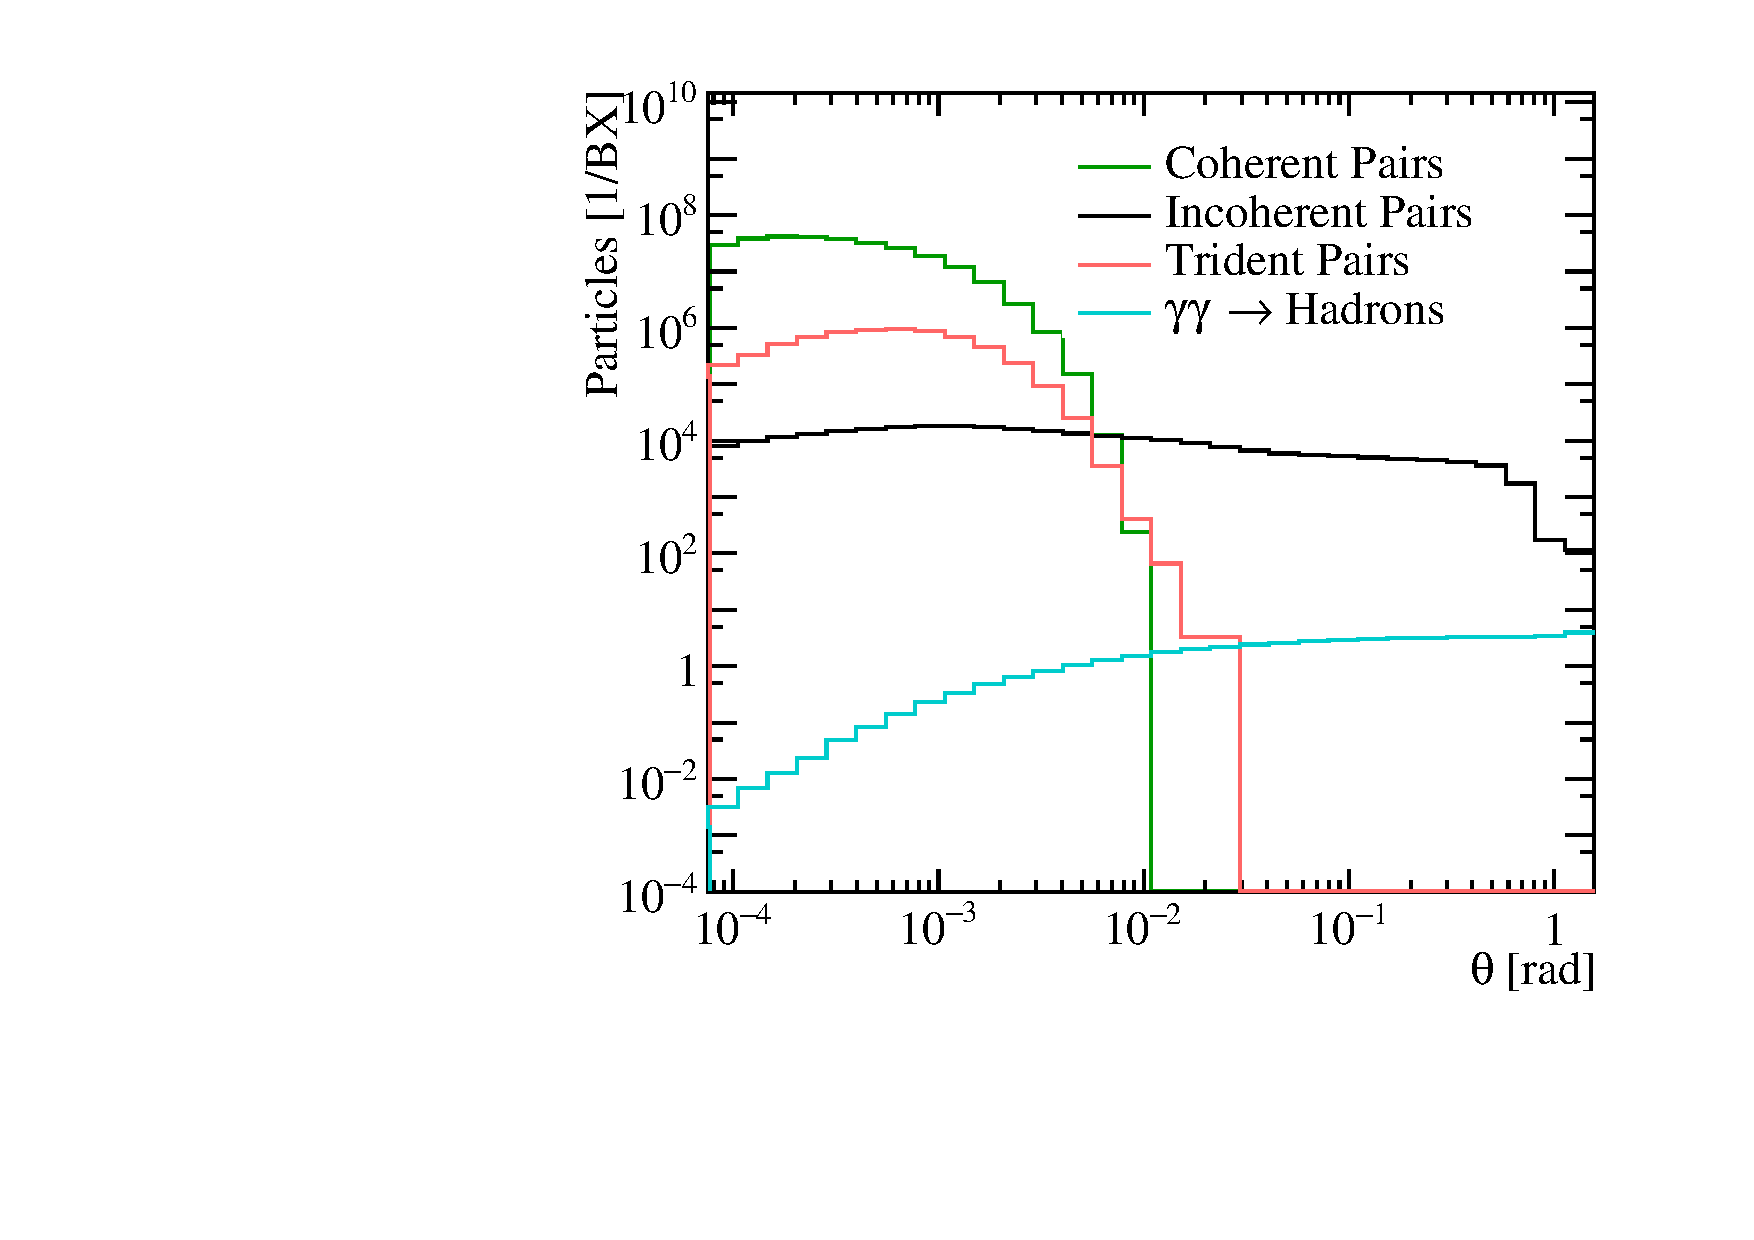
\includegraphics[width=0.5\textwidth]{Introduction/Plots/CDRPlots/BackgroundAngleCut.pdf}
\caption[Angular distribution of number of particles for beam induced backgrounds for CLIC at $\sqrt{s}=3$~TeV.  Figure taken from \cite{Linssen:2012hp}.]{Angular distribution of number of particles for beam induced backgrounds for CLIC at $\sqrt{s}=3$~TeV.  Figure taken from \cite{Linssen:2012hp}.}
\label{fig:backgroundangle}
\end{figure}

The dominant beam-related background found at the CLIC experiment is $\gamma\gamma \rightarrow hadrons$.  Table \ref{table:clicbkgsummary} shows that $\gamma\gamma \rightarrow hadrons$ backgrounds deposit more energy within the detector than the incoherent pair production.  Each bunch crossing for CLIC at $\sqrt{s}=3$~TeV contains an average of 3.2 $\gamma\gamma \rightarrow hadrons$ events and $3\times10^{5}$ incoherent pairs, however, the vast majority of incoherent pairs are produced with low transverse momenta and are collinear with the outgoing beam.

\begin{table}[h!]
\centering
\begin{tabular}{ l r r }
\hline
Subdetector & Incoherent Pairs [TeV] & $\gamma\gamma \rightarrow hadrons$ [TeV] \\ 
\hline
ECal Endcaps & 2 & 11 \\
ECal Barrel & - & 1.5 \\
HCal Endcaps & 16 & 6 \\
HCal Barrel & 0 & 0.3 \\
\hline
Total Calorimeter & 18 & 19 \\
\hline
Central Tracker & - & 7 \\ 
\hline
\end{tabular}
\caption[Summary of the background conditions at $\sqrt{s}=3$~TeV for the CLIC\_ILD detector model.  The numbers correspond to the background for an entire CLIC bunch train, i.e. 312 bunch crossings separated by a 0.5~ns gap.  The reconstructed calorimeter energies are integrated over 300~ns from the start of the bunch train. The backgrounds in the HCal from incoherent pairs are pessimistic as no attempts to mitigate the effect of neutrons from incoherent pair interactions in the BeamCal have been made.  Figure taken from \cite{Linssen:2012hp}.]{Summary of the background conditions at $\sqrt{s}=3$~TeV for the CLIC\_ILD detector model.  The numbers correspond to the background for an entire CLIC bunch train.  The reconstructed calorimeter energies are integrated over 300~ns from the start of the bunch train. The backgrounds in the HCal from incoherent pairs are pessimistic as no attempts to mitigate the effect of neutrons from incoherent pair interactions in the BeamCal have been made.  Figure taken from \cite{Linssen:2012hp}.}
\label{table:clicbkgsummary}
\end{table}

%========================================================================================
%========================================================================================

%Physics introduction leading to chapter description.
%Max 2-3 pages
%Standard model extremely successful, missing gravity though
%Higgs discovery added crucial piece for mass generation
%Properties missing:
%Dark matter coupling
%CP violation -> Matter > antimatter
%ILC designed to study Higgs at 125 GeV, e+e-->Zh peak cross section at 250 GeV allows decay of Higgs to be measured by recoil of Z
%Top quark mass also studies.  Heaviest particle so coupling to H will be strong.
%Ultra-Precision for EW sector, which is only known CP violation 
%CLIC EW symmetry breaking at TeV scale
%and SUSY searches
%Improvement to LHC
%Precision Quantitative improvement of what is know , Jump in physics e.g. GUT in SUSY only proposed from precision EW  Lightness of Higgs from LEP electroweak data
%Discovery reach from processes with low production cross section at LHC
%Precision from PFlow
%Chapter Vertex
%Chapter Energy Est
%Chapter Calo Opt
%Chapter Physics Analysis
%========================================================================================